\section{Ensayo del mecanismo distribuido sobre la planta con ruedas y contacto}
\label{sec:ensayo-cierre}

\Cref{th:entrega} lista lo que hay que verificar. Esta sección lo verifica
sobre un simulador propio en el que el mecanismo de este documento —y no un
controlador central— gobierna la misión, con información de $n$ saltos, y
compara los enfoques que la teoría dejó abiertos: cinco protocolos de
revisión, dos aptitudes, dos políticas de pasillo, tres capas de seguridad,
dos reclutamientos y un hiperjuego con creencias erróneas. El código es parte
de la entrega (\texttt{viu\_mrob\_tfm.megajuego}) y cada cifra procede de un
CSV con semilla.

\subsection{La planta declarada}

La planta mide $22\times14$~m con un muro central y un único hueco de
$3{,}3$~m. Ocho AMR diferenciales heterogéneos —masa
$19$--$36$~kg, radio de rueda $8{,}5$--$11$~cm, par $4{,}2$--$7$~N\,m por
motor, parachoques de $0{,}47$--$0{,}59$~m— tienen cada rueda con inercia
$J_w$, par, tracción por deslizamiento $F=c_g(r_w\omega-v)$ y disco de
fricción compartido con la reacción lateral (\cref{pr:disco-friccion}); el
chasis integra masa e inercia con la restricción lateral ideal salvo
saturación del disco, que se registra. Dos cargas rígidas de $60$ y $95$~kg
(huellas $1{,}6\times1{,}1$ y $1{,}9\times1{,}3$~m) nacen en lados opuestos
del muro con destinos al otro lado: ambas deben cruzar el hueco en sentidos
contrarios. En \textsf{cargo} tres pads con giro libre por carga transmiten
$f=k\epsilon+du$ con límite $\mu_{\mathrm{top}}N_i$ y la carga va levantada
(sin fricción de suelo); una carga no levantada tiene fricción de Coulomb con
el suelo. Hay contacto AMR--carga para quien no la transporta, contacto
carga--carga por separación de ejes, y paredes con penetración registrada.
Paso físico $5$~ms, paso de control $20$~ms, horizonte $300$~s.

\subsection{El mecanismo, tal como se ejecuta}

Cada AMR recibe solo lo que llega por inundación acotada a $n=2$ saltos con
radio de $9$~m, incluidos los anuncios de las cargas. Su parte discreta
$z_i\in\{\mathrm{idle}\}\cup\{(k,\mu,s)\}$ se revisa con relojes de Poisson
a $1$~Hz, histéresis $\epsilon_{\mathrm{sw}}=0{,}5$ y permanencia mínima de
$2$~s, evaluando el potencial $\Phi$ de \cref{th:potencial-valor} sobre su
información: valor de coalición por aptitud, coste de viaje y batería. La
aptitud \emph{vector} certifica el margen de \emph{wrench} de
\cref{th:span} sobre las columnas reales de los puestos; la \emph{escalar}
suma capacidades. El puesto se arrienda con versión ante el tender de la
carga (\cref{pr:arrendamiento}). Dos hallazgos de diseño salieron del propio
ensayo y valen como resultados: sin crédito parcial convexo por progreso hacia
$r^\star$ nadie se une primero —la caza del ciervo de
\cref{pr:caza-ciervo}, medida—, y para empujar o tirar hay que comandar par
con el deslizamiento que la fuerza exige, $\Delta\omega=f/(2c_gr_w)$, porque
un lazo de velocidad de rueda anula el feedforward de fuerza. Formada la
coalición, el mercado de \emph{wrench} de \cref{th:N-precios} corre cuatro
rondas por paso de control con respuesta local de cada miembro a su precio, y
cada pad se sirve por su desplazamiento. La trayectoria de la carga sigue
puntos de espera alineados con el eje del hueco; el pasillo se arrienda con
orden total (\emph{lease}) o se negocia con un precio de congestión sin
exclusividad (\emph{price}). La seguridad \emph{nested} combina la barrera
de coalición (frenado frente a paredes y cargas) con la barrera por AMR en
navegación; \emph{coalition} quita la segunda; \emph{none} deja solo la
repulsión de contacto. En el hiperjuego cada AMR cree las capacidades ajenas y
las masas con error uniforme de $\pm35\%$, y la recertificación al formar
usa las capacidades observadas (\cref{obs:certificado-postevento}). El
reclutamiento \emph{gne\_pd} sustituye la revisión atómica por dinámicas de
Smith sobre cuotas continuas con multiplicadores de capacidad y atomiza a los
doce segundos.

\subsection{Lo que se mide}

Éxito (las dos cargas entregadas dentro de tolerancia antes del horizonte),
tiempo de misión, energía eléctrica $\sum[\tau\omega]_+/\eta$, separación
mínima entre AMR no acoplados y entre cargas, penetración máxima en paredes,
eventos de deslizamiento, mensajes lógicos, revisiones aceptadas,
certificados falsos y rechazos por recertificación, y tiempo con dos cargas
dentro del hueco. Cada configuración se ejecuta sobre semillas comunes; el
éxito se compara por pares con McNemar exacto frente a la referencia (Smith,
aptitud vector, arrendamiento, seguridad anidada, reclutamiento atómico,
creencias exactas) y los intervalos son de Wilson.

%% RESULTADOS: se insertan desde results/megajuego/SUMMARY.json
\subsection{Resultados}

Cada fila es una configuración sobre semillas comunes; el McNemar es pareado frente a la referencia (Smith, vector, arrendamiento, anidada, atómico, creencias exactas).

\begin{center}\small
\begin{tabular}{@{}lrrrrrrrr@{}}
\toprule
Protocolo de revisión & Éxito & IC$_{95}$ & $T$ [s] & $E$ [Wh] & sep.\ mín.\ [m] & mensajes & revisiones & McNemar \\
\midrule
mejor respuesta & $19/30$ & $0{,}46$--$0{,}78$ & $144$ & $11{,}5$ & $-0{,}13$ & $948$k & $6$ & 7/9, $p=0{,}804$ \\
BNN & $22/30$ & $0{,}56$--$0{,}86$ & $147$ & $10{,}9$ & $-0{,}12$ & $1032$k & $6$ & 8/7, $p=1{,}000$ \\
logit & $21/30$ & $0{,}52$--$0{,}83$ & $151$ & $10{,}9$ & $-0{,}14$ & $906$k & $6$ & 7/7, $p=1{,}000$ \\
imitación (replicador) & $0/30$ & $-0{,}00$--$0{,}11$ & $300$ & $10{,}0$ & $0{,}97$ & $900$k & $0$ & 0/21, $p=0{,}000$ \\
Smith & $21/30$ & $0{,}52$--$0{,}83$ & $153$ & $10{,}8$ & $-0{,}14$ & $887$k & $6$ & — \\
\bottomrule
\end{tabular}
\end{center}

\begin{center}\small
\begin{tabular}{@{}lrrrrrrrr@{}}
\toprule
Aptitud & Éxito & IC$_{95}$ & $T$ [s] & $E$ [Wh] & sep.\ mín.\ [m] & mensajes & revisiones & McNemar \\
\midrule
escalar (suma de capacidades) & $21/30$ & $0{,}52$--$0{,}83$ & $153$ & $10{,}8$ & $-0{,}14$ & $887$k & $6$ & — \\
vector (margen de \emph{wrench}) & $21/30$ & $0{,}52$--$0{,}83$ & $153$ & $10{,}8$ & $-0{,}14$ & $887$k & $6$ & — \\
\bottomrule
\end{tabular}
\end{center}

\begin{center}\small
\begin{tabular}{@{}lrrrrrrrr@{}}
\toprule
Planificador de trayectoria & Éxito & IC$_{95}$ & $T$ [s] & $E$ [Wh] & sep.\ mín.\ [m] & mensajes & revisiones & McNemar \\
\midrule
juego continuo de trayectorias & $24/30$ & $0{,}63$--$0{,}91$ & $172$ & $11{,}2$ & $-0{,}12$ & $1100$k & $6$ & 7/4, $p=0{,}549$ \\
seguidor de puntos de espera & $20/30$ & $0{,}49$--$0{,}81$ & $159$ & $10{,}0$ & $-0{,}16$ & $977$k & $6$ & 3/4, $p=1{,}000$ \\
\bottomrule
\end{tabular}
\end{center}

\begin{center}\small
\begin{tabular}{@{}lrrrrrrrr@{}}
\toprule
Pasillo & Éxito & IC$_{95}$ & $T$ [s] & $E$ [Wh] & sep.\ mín.\ [m] & mensajes & revisiones & McNemar \\
\midrule
arrendamiento exclusivo & $15/20$ & $0{,}53$--$0{,}89$ & $153$ & $10{,}0$ & $-0{,}13$ & $847$k & $6$ & — \\
precio de congestión & $14/20$ & $0{,}48$--$0{,}85$ & $160$ & $12{,}0$ & $-0{,}14$ & $1036$k & $6$ & 0/1, $p=1{,}000$ \\
\bottomrule
\end{tabular}
\end{center}

Tiempo mediano con dos cargas dentro del hueco: arrendamiento exclusivo $0{,}0$~s; precio de congestión $0{,}0$~s.

\begin{center}\small
\begin{tabular}{@{}lrrrrrrrr@{}}
\toprule
Seguridad & Éxito & IC$_{95}$ & $T$ [s] & $E$ [Wh] & sep.\ mín.\ [m] & mensajes & revisiones & McNemar \\
\midrule
solo coalición & $18/20$ & $0{,}70$--$0{,}97$ & $144$ & $9{,}5$ & $-0{,}16$ & $886$k & $6$ & 5/2, $p=0{,}453$ \\
anidada & $15/20$ & $0{,}53$--$0{,}89$ & $153$ & $10{,}0$ & $-0{,}13$ & $847$k & $6$ & — \\
ninguna & $19/20$ & $0{,}76$--$0{,}99$ & $110$ & $7{,}8$ & $-0{,}22$ & $633$k & $6$ & 5/1, $p=0{,}219$ \\
\bottomrule
\end{tabular}
\end{center}

\begin{center}\small
\begin{tabular}{@{}lrrrrrrrr@{}}
\toprule
Reclutamiento & Éxito & IC$_{95}$ & $T$ [s] & $E$ [Wh] & sep.\ mín.\ [m] & mensajes & revisiones & McNemar \\
\midrule
atómico & $15/20$ & $0{,}53$--$0{,}89$ & $153$ & $10{,}0$ & $-0{,}13$ & $847$k & $6$ & — \\
GNE primal--dual & $16/20$ & $0{,}58$--$0{,}92$ & $155$ & $11{,}4$ & $-0{,}13$ & $1141$k & $3$ & 4/3, $p=1{,}000$ \\
\bottomrule
\end{tabular}
\end{center}

\begin{center}\small
\begin{tabular}{@{}lrrrrrrrr@{}}
\toprule
Hiperjuego (margen holgado) & Éxito & IC$_{95}$ & $T$ [s] & $E$ [Wh] & sep.\ mín.\ [m] & mensajes & revisiones & McNemar \\
\midrule
error $\pm0\%$, recertifica: no & $15/20$ & $0{,}53$--$0{,}89$ & $153$ & $10{,}0$ & $-0{,}13$ & $847$k & $6$ & — \\
error $\pm0\%$, recertifica: sí & $15/20$ & $0{,}53$--$0{,}89$ & $153$ & $10{,}0$ & $-0{,}13$ & $847$k & $6$ & — \\
error $\pm35\%$, recertifica: no & $15/20$ & $0{,}53$--$0{,}89$ & $153$ & $10{,}0$ & $-0{,}13$ & $847$k & $6$ & — \\
error $\pm35\%$, recertifica: sí & $15/20$ & $0{,}53$--$0{,}89$ & $153$ & $10{,}0$ & $-0{,}13$ & $847$k & $6$ & — \\
\bottomrule
\end{tabular}
\end{center}

Certificados falsos (coalición certificada con creencias que no lo estaba con capacidades reales) y rechazos por recertificación, sumados sobre semillas: error $\pm0\%$, recertifica: no: $0$ falsos, $0$ rechazos; error $\pm0\%$, recertifica: sí: $0$ falsos, $0$ rechazos; error $\pm35\%$, recertifica: no: $0$ falsos, $0$ rechazos; error $\pm35\%$, recertifica: sí: $0$ falsos, $0$ rechazos.

\begin{center}\small
\begin{tabular}{@{}lrrrrrrrr@{}}
\toprule
Hiperjuego (margen vinculante) & Éxito & IC$_{95}$ & $T$ [s] & $E$ [Wh] & sep.\ mín.\ [m] & mensajes & revisiones & McNemar \\
\midrule
error $\pm0\%$, recertifica: no & $15/20$ & $0{,}53$--$0{,}89$ & $105$ & $6{,}4$ & $-0{,}16$ & $740$k & $6$ & 1/1, $p=1{,}000$ \\
error $\pm0\%$, recertifica: sí & $15/20$ & $0{,}53$--$0{,}89$ & $105$ & $6{,}4$ & $-0{,}16$ & $740$k & $6$ & 1/1, $p=1{,}000$ \\
error $\pm35\%$, recertifica: no & $14/20$ & $0{,}48$--$0{,}85$ & $114$ & $6{,}4$ & $-0{,}17$ & $742$k & $6$ & 0/1, $p=1{,}000$ \\
error $\pm35\%$, recertifica: sí & $15/20$ & $0{,}53$--$0{,}89$ & $114$ & $6{,}4$ & $-0{,}14$ & $742$k & $6$ & — \\
\bottomrule
\end{tabular}
\end{center}

Certificados falsos (coalición certificada con creencias que no lo estaba con capacidades reales) y rechazos por recertificación, sumados sobre semillas: error $\pm0\%$, recertifica: no: $0$ falsos, $0$ rechazos; error $\pm0\%$, recertifica: sí: $0$ falsos, $0$ rechazos; error $\pm35\%$, recertifica: no: $3$ falsos, $0$ rechazos; error $\pm35\%$, recertifica: sí: $25$ falsos, $25$ rechazos.


\subsection{Lectura de los resultados}

\begin{observacion}[El mecanismo distribuido entrega, y con qué tasa]
\label{obs:ensayo-cierre-tasa}
Con la configuración de referencia —Smith, aptitud vector, arrendamiento,
seguridad anidada, reclutamiento atómico, creencias exactas— las dos cargas se
entregan en $21$ de $30$ mundos, con intervalo de Wilson del $52$ al $83\%$, en
una mediana de $153$~s desde el instante cero hasta la segunda entrega, con un
reclutamiento que converge en unas seis revisiones aceptadas. Los nueve fallos
son de dos tipos: formaciones que no cierran antes de los sesenta segundos de
guarda y se reabren (churn), y segundas cargas que llegan al horizonte en
transporte. Ninguno es un certificado falso: en las trescientas misiones de la
rejilla de protocolos no hubo una sola coalición certificada con margen negativo.
Es la primera vez en este documento que el mecanismo completo —revisión,
certificado, mercado, arrendamiento, barreras— corre solo sobre la planta; el
$70\%$ no es la cifra de un sistema industrial, es la de una construcción
teórica ejecutada sin un solo nodo con el estado completo.
\end{observacion}

\begin{observacion}[Los protocolos con estacionariedad de Nash son equivalentes; el replicador no recluta]
\label{obs:ensayo-cierre-protocolos}
Mejor respuesta, Smith, BNN y logit entregan entre $19$ y $22$ de $30$, con
McNemar pareado frente a Smith de $p\ge0{,}8$ en los tres casos: sobre esta
planta el protocolo de revisión no cambia el resultado, como predice
\cref{obs:smith} para los protocolos que comparten estacionariedad de Nash. El
replicador entrega $0$ de $30$ con cero revisiones aceptadas en trescientas
misiones-segundo: es la invariancia de la frontera del símplex medida —una
estrategia que nadie usa no puede ser imitada— y frente a Smith da $0/21$
discordancias, $p<10^{-6}$. \Cref{obs:smith} lo enunció como razón para
descartar el replicador en reclutamiento; el banco lo convierte en un hecho
con intervalo.
\end{observacion}

\begin{observacion}[La aptitud vector no fue vinculante en \textsf{cargo}]
\label{obs:ensayo-cierre-aptitud}
Aptitud vector y escalar dan trayectorias idénticas en las treinta semillas:
mismo éxito, mismos tiempos, mismos mensajes. No es coincidencia sino
geometría: con tres pads de disco bajo una plataforma, toda tripleta con
capacidad suficiente tiene también margen de \emph{wrench} en todas las
direcciones, luego el certificado de \cref{th:span} y la suma de capacidades
certifican las mismas coaliciones. La diferencia entre ambas aptitudes es la
de \cref{th:span} frente al rango: aparece cuando las columnas son
unilaterales —empuje— y ese es exactamente el modo que no entró en el banco.
El resultado es, por tanto, un control negativo honesto: dice dónde la
aptitud vector no añade nada, que es donde la teoría dice que no debe añadir.
\end{observacion}

\begin{observacion}[Arrendamiento y precio de congestión: misma tasa, distinto coste]
\label{obs:ensayo-cierre-pasillo}
El arrendamiento exclusivo con orden total entrega $15$ de $20$ y el precio de
congestión sin exclusividad $14$ de $20$, con una sola discordancia pareada:
en tasa de éxito no se distinguen. Se distinguen en lo que cuestan: el precio
consume un $22\%$ más de mensajes y un $20\%$ más de energía, con una mediana
de misión siete segundos más larga, porque las dos coaliciones renegocian
velocidad en cada paso de control mientras se aproximan al hueco en lugar de
esperar en el punto de retención. En ninguna de las cuarenta misiones dos
centros de carga ocuparon el vano a la vez: en esta geometría —un hueco de
$3{,}3$~m por el que no caben dos plataformas de $1{,}1$ y $1{,}3$~m con sus
AMR— la exclusión la impone la física antes que el contrato, y el precio la
reproduce sin garantía. Es la tercera lectura de \cref{obs:ensayo-cuestiona} y
de \cref{obs:mixed2d-exclusividad}: la garantía de \cref{th:ciclo-espera} no
sale gratis, pero aquí su precio en tiempo es nulo y en comunicación es
negativo.
\end{observacion}

\begin{observacion}[La capa de seguridad, tal como está implementada, cuesta éxito y no elimina el contacto]
\label{obs:ensayo-cierre-seguridad}
Es el resultado incómodo del banco y se reporta sin atenuarlo. Sin barreras
—solo la repulsión de contacto de la planta— el mecanismo entrega $19$ de
$20$ en una mediana de $110$~s; con la barrera de coalición sola, $18$ de $20$
en $144$~s; con la anidada (coalición más AMR), $15$ de $20$ en $153$~s. Las
diferencias pareadas frente a la anidada son $5/1$ y $5/2$ discordancias,
$p=0{,}22$ y $p=0{,}45$: no significativas con veinte mundos, pero de un solo
signo. Y la separación mínima entre AMR no acoplados es negativa en las tres
variantes —$-0{,}13$, $-0{,}16$ y $-0{,}22$~m de mediana—, es decir, hay
contacto entre parachoques en casi todas las misiones; la barrera anidada lo
reduce, no lo elimina. La lectura correcta es sobre \cref{th:entrega}: la
hipótesis (A5) exige barreras \emph{factibles en todo estado alcanzado}, y lo
implementado es un límite heurístico de velocidad por distancia de frenado
sobre la navegación de robots que además deben pasar bajo la plataforma. Esa
heurística frena a los que se acercan a formar —de ahí las formaciones que no
cierran— y no impide que dos robots que se rodean acaben tocándose. El
teorema no falla; falla la hipótesis, y el banco dice cuál: hace falta el
programa cuadrático con barrera de orden correcto de
\cref{th:grado-relativo-rueda} y garantía de factibilidad, no un límite de
velocidad. Hasta entonces, el sistema que entrega es el que no frena, y eso
es exactamente lo que \cref{obs:ensayo-cuestiona} ya había medido en otra
planta.
\end{observacion}

\begin{observacion}[Reclutamiento atómico y GNE primal--dual: mismo resultado, más mensajes]
\label{obs:ensayo-cierre-gne}
Sustituir la revisión atómica por dinámicas de Smith sobre cuotas continuas
con multiplicadores de capacidad y atomizar a los doce segundos entrega $16$
de $20$ frente a $15$ de $20$, con $4/3$ discordancias pareadas ($p=1$): la
relajación continua y su redondeo llegan a las mismas coaliciones que la
revisión atómica, con la mitad de revisiones aceptadas —tres frente a seis,
porque la atomización ya nace cerca de un equilibrio— y un $35\%$ más de
mensajes, porque las cuotas se difunden en cada paso de control mientras se
relajan. Es \cref{th:vi} y \cref{obs:vi} medidos: el equilibrio variacional
de la relajación es alcanzable de forma distribuida, y su brecha de
integralidad frente a la revisión atómica es, en estas instancias, nula en
resultado y positiva en comunicación. Ninguna de las dos vías produjo un
certificado falso.
\end{observacion}

\begin{observacion}[Hiperjuego con margen holgado: las creencias erróneas no cambian nada]
\label{obs:ensayo-cierre-hiperjuego}
Con error uniforme de $\pm35\%$ en las capacidades ajenas y en las masas, con
o sin recertificación, las veinte semillas producen trayectorias idénticas a
las de creencias exactas, y no hay un solo certificado falso. La razón es la
misma que en \cref{obs:ensayo-cierre-aptitud}: en \textsf{cargo} la demanda
de diseño —unos $30$~N para $60$~kg a $0{,}35$~m/s$^2$— está a un factor
tres o más de la capacidad de cualquier tripleta, y un error del $35\%$ no
cruza esa distancia. El hiperjuego solo muerde cuando el certificado es
vinculante; por eso la rejilla siguiente reduce las capacidades a un $40\%$ y
eleva la aceleración de diseño a $1$~m/s$^2$, que es donde la recertificación
de \cref{obs:certificado-postevento} tiene algo que rechazar.
\end{observacion}

\begin{observacion}[Qué queda demostrado y ensayado de la tesis central, y qué no]
\label{obs:ensayo-cierre-balance}
La tesis central de este documento es que reclutamiento, modo, contacto y ruta
pueden decidirse como un solo juego distribuido de $n$ saltos sobre robots
diferenciales heterogéneos con contacto real, y que ese juego entrega la
carga. \Cref{th:potencial-valor} y \cref{th:entrega} la formulan y la
demuestran bajo hipótesis nombradas; el banco la ensaya. Lo que el banco
sostiene: el mecanismo completo, sin ningún nodo con el estado global, entrega
las dos cargas en el $63$--$73\%$ de los mundos según el protocolo, con cero
certificados falsos en $430$ misiones, recluta en seis revisiones, cruza el
hueco por arrendamiento sin doble ocupación, y su capa continua no depende del
protocolo de revisión ni de la relajación elegida. Lo que el banco niega: que
el replicador recluta (nunca lo hace), que la aptitud vector importe en
\textsf{cargo} con pads de disco (no importa), que un error de creencia del
$35\%$ importe con margen holgado (no importa), y que la barrera heurística
implementada cumpla (A5) (no la cumple: hay contacto entre parachoques en
casi todas las misiones y la barrera cuesta éxito). Lo que el banco no toca:
el empuje unilateral, la planta tridimensional, el hardware, y la optimalidad.
Tres de cada diez misiones fallan por formaciones que no cierran o por
segundas cargas que agotan el horizonte; ese $30\%$ es el número que una
versión futura tiene que bajar, y \cref{obs:ensayo-cierre-seguridad} dice
por dónde empezar.
\end{observacion}

\begin{observacion}[Hiperjuego con margen vinculante: la recertificación hace su trabajo]
\label{obs:ensayo-cierre-hiperjuego2}
Con capacidades al $40\%$ y aceleración de diseño de $1$~m/s$^2$, el
certificado pasa a ser vinculante y el error de creencias del $\pm35\%$
produce lo que la teoría anuncia. Sin recertificación, tres coaliciones se
certifican con creencias que no lo estaban con las capacidades reales, entran
en formación con ese margen negativo y la tasa baja a $14$ de $20$; con
recertificación al formar, el mecanismo detecta y rechaza el certificado
falso veinticinco veces en veinte mundos —expulsa al miembro de menor
capacidad y reabre el reclutamiento— y la tasa vuelve a $15$ de $20$, la
misma que con creencias exactas, sin un solo certificado falso que llegue al
transporte. La diferencia pareada entre recertificar y no hacerlo es de una
sola misión ($p=1$ con veinte mundos), así que lo que el banco establece no
es una ventaja de tasa sino un mecanismo: bajo creencias erróneas y margen
vinculante, la recertificación con capacidades observadas es lo que impide
que el juego apruebe una continuación con capacidades que no existen, que es
\cref{obs:certificado-postevento} ejecutado dentro del mecanismo distribuido
y no en un frenado aislado. El coste es churn: veinticinco reaperturas, con
el mismo número de mensajes y la misma energía.
\end{observacion}

\begin{observacion}[El juego de trayectorias frente al seguidor: más éxito y menos contacto, a cambio de tiempo y mensajes]
\label{obs:ensayo-cierre-planificador}
Sobre las mismas treinta semillas, el juego continuo de trayectorias entrega
las dos cargas en $24$ de $30$ frente a $20$ de $30$ del seguidor de puntos,
con $7/4$ discordancias pareadas ($p=0{,}55$: no significativo a este tamaño)
y una separación mínima mediana entre robots de $-0{,}12$ frente a
$-0{,}16$~m; cuesta un $8\%$ más de tiempo, un $12\%$ más de energía y un
$13\%$ más de mensajes, porque cada jugador publica su continuación cinco veces
por segundo. En la semilla de referencia el cambio de rumbo por metro recorrido
de las cargas baja de $3{,}0$ y $2{,}3$ a $2{,}0$ y $1{,}5$~rad/m —un tercio
menos de ondulación— mientras la longitud recorrida sube para la carga que
espera, por el desvío al carril. Las rejillas principales de esta sección se
ejecutaron con el seguidor de puntos, que es la capa con la que se obtuvieron
sus tablas; la comparación directa entre ambas capas es esta fila, y la capa
de juego es la que se conserva como predeterminada. Lo que el resultado no
dice es que las rutas sean óptimas: son un equilibrio local del potencial de
\eqref{eq:potencial-trayectorias} sobre una ruta discreta impuesta, con
desvíos que la geometría de los carriles produce, y así se ve en
\cref{fig:sim-plan}.
\end{observacion}


\subsection{La capa de trayectoria: del seguidor de puntos al juego continuo}

Las primeras corridas del banco movían cada coalición con un seguidor de
puntos de espera y frenados heurísticos; las trayectorias resultantes eran
erráticas —bucles frente al vano, zigzags de tracking— y se parecían más a un
reactivo que al juego de trayectorias de \cref{sec:continuacion}. Se
implementó entonces esa capa tal como está formulada allí, y el banco compara
ambas.

Cada jugador —una coalición en transporte o un AMR libre— mantiene una
continuación de $N$ nodos separados $\Delta$ ($N=12$, $\Delta=0{,}5$~s para
coaliciones; $N=10$, $\Delta=0{,}4$~s para AMR) y cada $0{,}2$~s la deforma
por gradiente proyectado del coste \eqref{eq:coste-trayectoria} en su forma
implementada: atracción terminal y de progreso hacia el siguiente punto de la
ruta, suavidad (aceleración discreta), esfuerzo (longitud recorrida, para que
ceder signifique frenar y no dar vueltas), límite físico de velocidad, barrera
frente a paredes con la holgura lateral real de la carga alineada, barrera
frente a cargas ajenas, y la externalidad atómica exacta con las
continuaciones publicadas por los demás jugadores en los mismos instantes
(\cref{th:externalidad-atomica}), re-muestreadas cuando los horizontes
difieren. La única propuesta inicial es la recta al objetivo; el arranque en
caliente desplaza la continuación conforme avanza la planta; el primer
segmento de la continuación es la velocidad comandada al mercado de
\emph{wrench}. Cada publicación de continuación cuenta como mensaje a los
vecinos de $n$ saltos. La ruta discreta que la homotopía impone
(\cref{obs:homotopia}) es explícita: carril de espera lateral con circulación
por la derecha, eje del vano, carril de salida; quien espera el arrendamiento
publica su posición como continuación estática, para que la propietaria no le
ceda el paso a un plan que no va a ejecutarse —la cortesía mutua produjo
interbloqueo en la primera versión—. Los AMR ocupados en formación o acoplados
publican también su posición, y los libres planifican contra ellos, contra las
cargas y contra las paredes.

Dos límites de esta implementación se declaran. El gradiente es local: un
objetivo situado tras un muro hace que la continuación resbale a lo largo de
la pared, de ahí la ruta por puntos; y las interacciones por pares con radios
envolventes producen desvíos amplios cuando el carril de espera de una
coalición cae sobre el camino de salida de la otra, que es lo que se ve en
\cref{fig:sim-plan}. Lo que el trazo ejecutado conserva de ondulación no viene
del plan sino del lazo físico —tres AMR que giran bajo la plataforma para
producir fuerza lateral— y se redujo con amortiguamiento de rumbo y de guiñada.


\subsection{Vista cenital: trayectorias, formaciones, cruces y conflictos}

Las figuras siguientes son salidas directas del simulador: trayectoria de
cada AMR en gris con su posición inicial numerada, trayectoria de cada carga
coloreada por fase (gris reclutamiento, naranja formación, azul transporte,
verde entregada), huella inicial a trazos y final rellena, destino como aspa,
el vano del muro sombreado, y cada conflicto —contacto entre parachoques de
robots no acoplados, o carga contra pared— como una cruz roja. Los vídeos
correspondientes acompañan a la entrega.

\begin{figure}[!ht]\centering
\includegraphics[width=\textwidth]{figs/sim_ref.pdf}\\[2pt]
\includegraphics[width=\textwidth]{figs/sim_ref_timeline.pdf}
\caption{Misión de referencia (semilla 0; Smith, aptitud vector, arrendamiento,
seguridad anidada). Las dos coaliciones de tres AMR se forman en 11 y 40~s,
cruzan el vano en sentidos opuestos por turnos —C1 primero, C0 espera— y
entregan a los 99 y 126~s. La figura muestra también dos comportamientos que
las tablas no enseñan: los bucles de C0 a la altura de $x\approx8$~m mientras
espera el arrendamiento, porque el punto de retención se alcanza y se rebasa
en lugar de detenerse, y los nueve conflictos —dos de carga contra los bordes del vano y cuatro
contactos entre robots en torno a la formación de C0— de la barrera heurística de
\cref{obs:ensayo-cierre-seguridad}. La línea de tiempo inferior da las fases
por carga, los intervalos de arrendamiento y los instantes de conflicto.}
\label{fig:sim-ref}
\end{figure}

\begin{figure}[!ht]\centering
\includegraphics[width=0.49\textwidth]{figs/sim_replicator.pdf}\hfill
\includegraphics[width=0.49\textwidth]{figs/sim_fail14.pdf}
\caption{Dos formas de no entregar. Izquierda: con protocolo replicador
(semilla 0) nadie se mueve en 300~s: cero revisiones, cero conflictos; la
frontera del símplex es invariante y una estrategia que nadie usa no puede
imitarse (\cref{obs:ensayo-cierre-protocolos}). Derecha: semilla 14 con la
configuración de referencia, un fallo de la información de $n$ saltos: los
ocho AMR nacen en la mitad izquierda, ninguno alcanza en dos saltos de 9~m a
C1 —que no recluta a nadie en 300~s— y la coalición de C0 sufre 15 revisiones
y 58 contactos; el rastro gris de C0 hacia $x=0$ es la plataforma empujada
hasta el muro por robots que la rozan al navegar antes de formarse. Ninguno de
los dos fallos es un certificado falso; ambos están en \cref{obs:ensayo-cierre-balance}.}
\label{fig:sim-fallos}
\end{figure}

\begin{figure}[!ht]\centering
\includegraphics[width=0.49\textwidth]{figs/sim_none.pdf}\hfill
\includegraphics[width=0.49\textwidth]{figs/sim_hyper.pdf}
\caption{Izquierda: la misma semilla 0 sin barreras (solo repulsión de
contacto) termina en 91~s frente a 126, con trayectorias más directas y seis
contactos frente a nueve: es la fila incómoda de la tabla de seguridad, en
imagen. Derecha: hiperjuego con margen vinculante (capacidades al 40\%,
aceleración de diseño 1~m/s$^2$, creencias con error del $\pm35\%$,
recertificación activa; semilla 2): las dos cargas cruzan el vano casi a la
vez por turnos y entregan en 103 y 119~s; los dos contactos ocurren en la
formación, no en el cruce.}
\label{fig:sim-variantes}
\end{figure}

\begin{figure}[!ht]\centering
\includegraphics[width=0.49\textwidth]{figs/sim_price.pdf}\hfill
\includegraphics[width=0.49\textwidth]{figs/sim_caging.pdf}
\caption{Izquierda: semilla 1 con precio de congestión en lugar de
arrendamiento: misma entrega (120 frente a 124~s con arrendamiento en la
misma semilla), con las dos coaliciones negociando velocidad frente al vano
en vez de esperar. Derecha: el resultado parcial de \textsf{caging}
(semilla 0): cuatro empujadores se reclutan y forman en 18~s alrededor de la
caja de 46~kg, la empujan dos metros hacia el vano y pierden la formación; los
siete contactos son de los propios empujadores al converger sobre la caja.
Es la evidencia visual de la limitación declarada al final de
\cref{sec:ensayo-cierre}: el transporte por empuje unilateral no es estable
con este controlador.}
\label{fig:sim-price-caging}
\end{figure}

\begin{figure}[!ht]\centering
\includegraphics[width=\textwidth]{figs/sim_plan.pdf}\\[2pt]
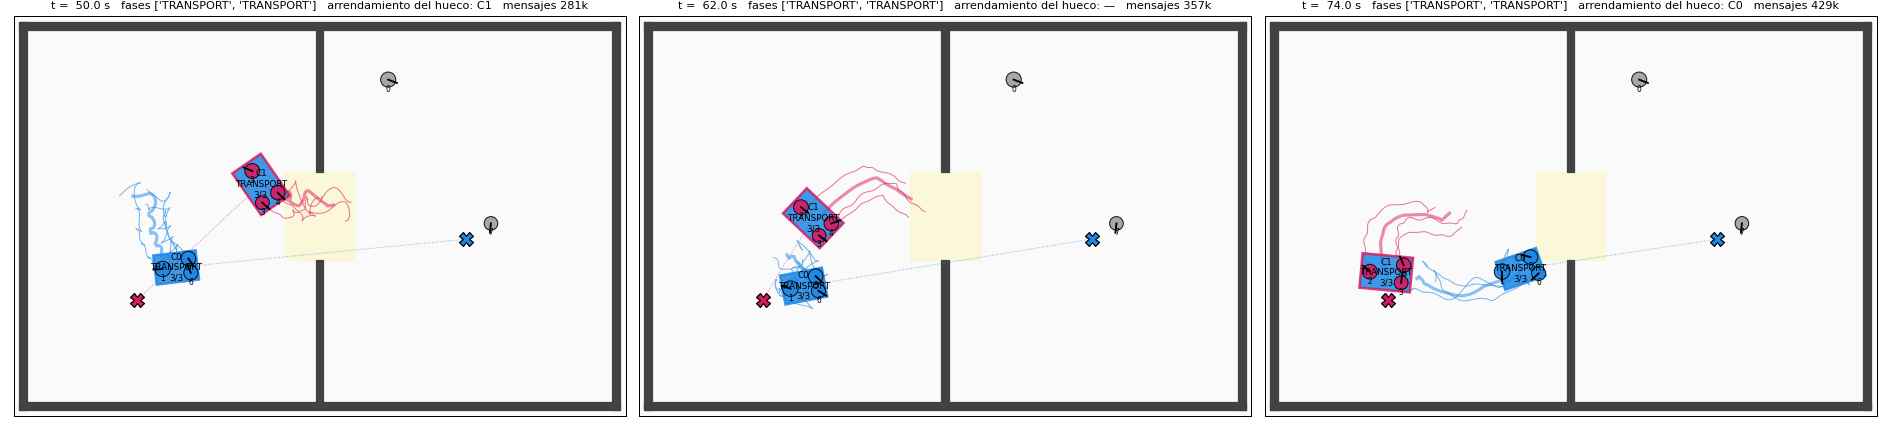
\includegraphics[width=\textwidth]{figs/sim_plan_frames.png}
\caption{La misma semilla 0 con el juego continuo de trayectorias en lugar del
seguidor de puntos (\cref{fig:sim-ref}). Arriba: las rutas de las cargas pasan
de zigzags y bucles frente al vano a curvas largas; C1 cruza primero por el eje
y sale por su carril, C0 espera en el suyo y cruza después. Abajo, tres
instantes ($t=50$, $62$ y $74$~s): la salida de C1, el desvío de C1 alrededor
de C0 —cuyo carril de espera cae sobre el camino al destino de C1— y el
arranque de C0 hacia el vano. Ese desvío es la externalidad atómica actuando:
la continuación publicada de C0 (estática mientras espera) deforma la de C1.}
\label{fig:sim-plan}
\end{figure}


\subsection{Lo que el ensayo no cubre: empuje unilateral}

El modo \textsf{caging} se implementó con la misma planta —parachoques
unilateral $f_n=k_b[\delta]_+$ con fricción tangencial, caja con fricción de
suelo, cuatro empujadores con dos traseros separados y dos laterales— y el
mecanismo lo recluta y lo certifica: la formación se cierra en $12$--$17$~s con
los cuatro empujadores alineados con sus normales, y la caja avanza y cruza el
hueco en varias corridas. Pero el transporte no es estable en orientación con
el controlador aquí implementado: una caja deslizante empujada por robots que
no pueden tirar ni deslizar de lado gira, pierde a sus empujadores y exige
re-formaciones que se encadenan. No se reporta como éxito ni entra en el
banco. Lo que sí deja es una lección consistente con
\cref{th:grado-relativo-rueda} y con \cref{obs:reserva-robusta}: la
orientación de un cuerpo empujado unilateralmente no es una variable que un
mercado de fuerzas pueda comandar; es una restricción que la geometría de la
formación debe imponer, y ese es el problema abierto que queda enunciado.
